\subsubsection{Rancangan Detail Data Collector}
\label{subsubsection:detail-data-collector}

Seperti yang sudah dijelaskan pada Bagian \ref{subsubsection:data-collector}, \textit{Data Collector} merupakan komponen yang bertanggung jawab untuk mengumpulkan data eksperimen dari sistem yang sedang diuji. Komponen ini berperan penting dalam menyediakan data yang diperlukan untuk analisis kinerja dan evaluasi sistem. Selain itu, \textit{Data Collector} juga menyediakan antarmuka yang memungkinkan pengguna untuk melakukan eksperimen dengan sistem menggunakan variabel jumlah \textit{virtual user}, ukuran data, \textit{bandwidth}, dan konfigurasi sistem yang digunakan. Ilustrasi struktur \textit{Data Collector} yang lebih detail dapat dilihat pada Gambar \ref{fig:data-collector-structure}.

\begin{figure}[ht]
	\centering
	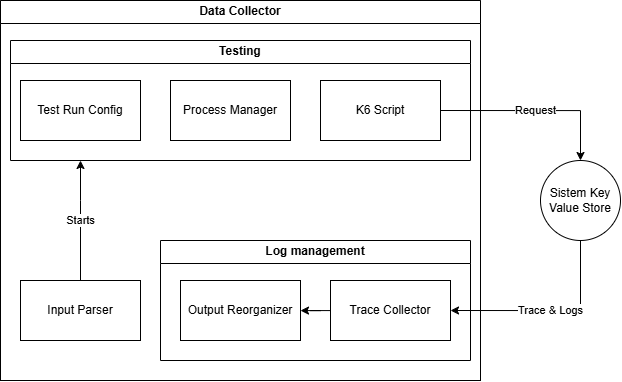
\includegraphics[width=0.75\textwidth]{resources/chapter-3/data-collector-architecture.png}
	\caption{Struktur Data Collector}
	\label{fig:data-collector-structure}
\end{figure}

Komponen internal yang ada pada \textit{Data Collector} adalah \textit{Input Parser} yang berfungsi untuk mem-parsing input dari pengguna dan \textit{Config Parser} yang berfungsi untuk membaca konfigurasi sistem yang digunakan dalam eksperimen untuk kemudian dibangun.